% ENLA Analysis Report
\documentclass[11pt, a4paper]{article}
\usepackage[T1]{fontenc}
\usepackage[utf8]{inputenc}
\usepackage{lmodern}
\usepackage[margin=1in]{geometry}
\usepackage{setspace}
\usepackage{graphicx}
\usepackage{caption}
\usepackage{subcaption}
\usepackage{booktabs}
\usepackage{longtable}
\usepackage{tabularx}
\usepackage{hyperref}
\usepackage{amsmath, amssymb}
\usepackage{siunitx}
\usepackage{xcolor}
\hypersetup{
  colorlinks=true,
  linkcolor=blue,
  citecolor=blue,
  urlcolor=blue
}
\setlength{\parskip}{0.6em}
\setlength{\parindent}{0pt}
\onehalfspacing

\title{ENLA Analysis Report\\\large Exploratory Data, Networks, and Causal Discovery}
\author{Francisco Richter}
\date{\today}

\begin{document}
\maketitle
% \tableofcontents % removed per request
\newpage

% ===================== INTRODUCTION =====================
\section{Introduction}
This report presents an integrated analysis of ENLA data combining Exploratory Data Analysis (EDA), correlation network exploration by questionnaire, and causal structure learning via the PC algorithm. We outline the data sources, preprocessing, and the rationale for the selected analytical pipeline.

% ===================== EDA =====================
\section{Exploratory Data Analysis}
We summarize the EM performance distributions and subgroup patterns. Below we present three side-by-side scatter-density (contour) plots for Gender, Language, and Area.

\begin{figure}[h]
  \centering
  % Gender
  \begin{subfigure}[t]{0.32\textwidth}
    \centering
    \IfFileExists{figures/eda_gender_contour.png}{%
      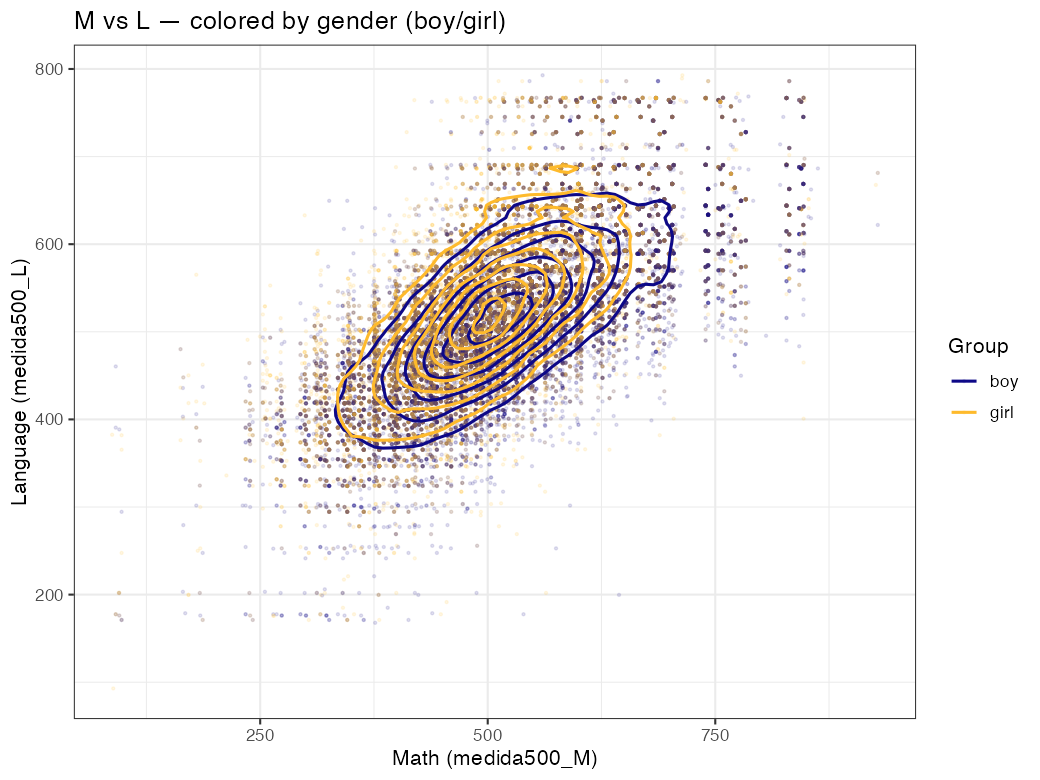
\includegraphics[width=\textwidth]{figures/eda_gender_contour.png}%
    }{%
      \fbox{\begin{minipage}[c][0.22\textheight][c]{\textwidth}\centering
      Placeholder: \texttt{figures/eda_gender_contour.png}
      \end{minipage}}%
    }
    \caption{Gender}
  \end{subfigure}
  \hfill
  % Language
  \begin{subfigure}[t]{0.32\textwidth}
    \centering
    \IfFileExists{figures/eda_language_contour.png}{%
      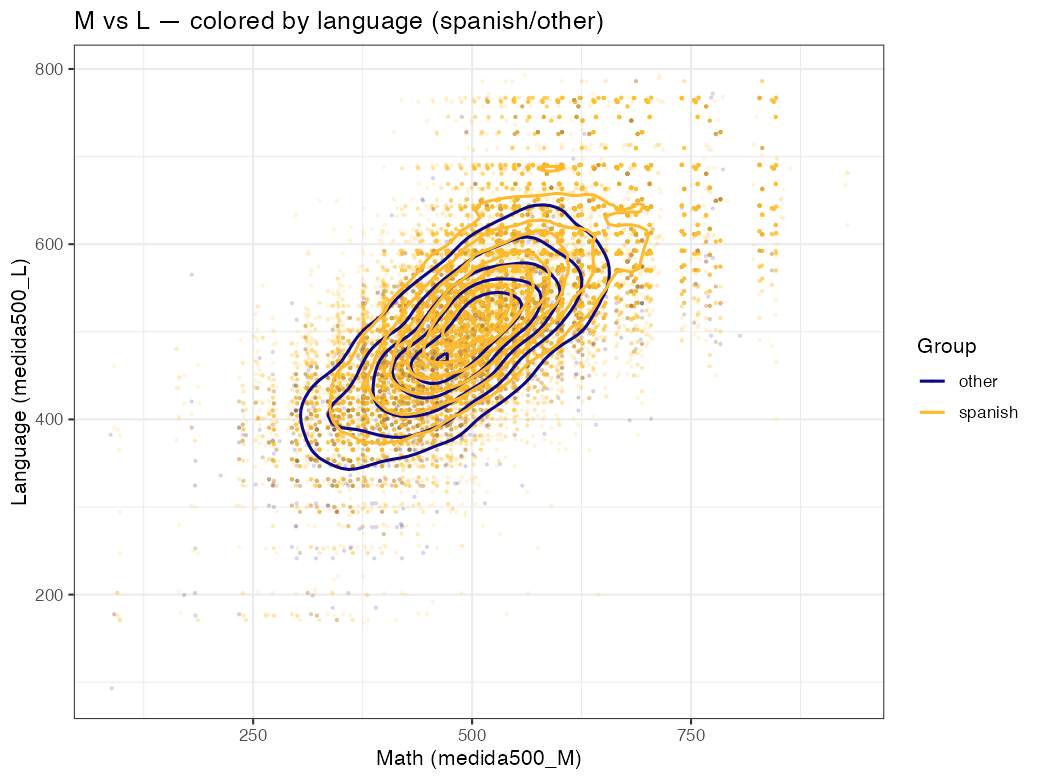
\includegraphics[width=\textwidth]{figures/eda_language_contour.png}%
    }{%
      \fbox{\begin{minipage}[c][0.22\textheight][c]{\textwidth}\centering
      Placeholder: \texttt{figures/eda_language_contour.png}
      \end{minipage}}%
    }
    \caption{Language}
  \end{subfigure}
  \hfill
  % Area (replacing school)
  \begin{subfigure}[t]{0.32\textwidth}
    \centering
    \IfFileExists{figures/eda_area_contour.png}{%
      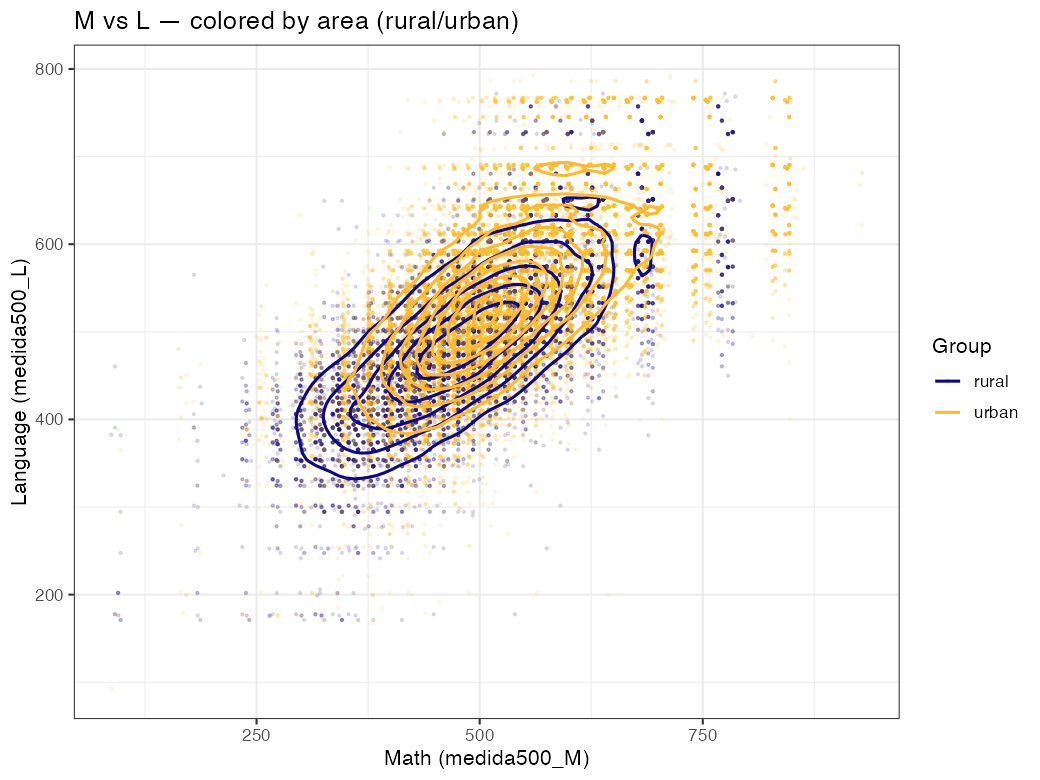
\includegraphics[width=\textwidth]{figures/eda_area_contour.png}%
    }{%
      \fbox{\begin{minipage}[c][0.22\textheight][c]{\textwidth}\centering
      Placeholder: \texttt{figures/eda_area_contour.png}
      \end{minipage}}%
    }
    \caption{Area}
  \end{subfigure}
  \caption{Scatter with 2D-density contours: Math vs. Language by subgroup.}
\end{figure}

\paragraph{Findings.}
Across the three subgroupings we observe clear distributional shifts in performance (Math vs. Language):

\begin{itemize}
  \item \textbf{Gender.} The lower tail (low-performance students) is broadly similar between boys and girls, suggesting comparable density of lower scores. However, the upper tail differs: high-performance students, especially in Mathematics, concentrate more among boys. This is visible as higher-density contours for boys in the top-right region of the plot.
  \item \textbf{Language.} When stratifying by first language, the entire joint distribution appears shifted in favor of Spanish speakers relative to indigenous languages. This reflects both a higher central tendency and a greater mass of high performers among Spanish speakers.
  \item \textbf{Area.} A similar whole-distribution shift is present by area, favoring urban over rural contexts. The effect is not restricted to the extremes; rather, the bulk of the distribution is translated toward better performance in urban areas.
\end{itemize}


\clearpage

% ===================== CORRELATION AND NETWORK ANALYSIS =====================
\section{Correlation and Network Analysis}
We examine pairwise (Pearson) correlation networks constructed from questionnaire items. Items are grouped by construct (pXX and pXX\_YY), and edges indicate absolute correlations above an analysis threshold (with pairwise-complete observations). We focus on:
\begin{itemize}
  \item \textbf{Overall connectivity and hubs:} constructs that act as hubs may reflect broad latent factors.
  \item \textbf{Links to outcomes (L/M):} strong positive or negative correlations to Language (L) or Math (M) highlight salient relationships visible at the association level.
  \item \textbf{Source-specific patterns:} differences across questionnaires (e.g., Familia vs. Docente) point to context-specific relationships.
\end{itemize}


% ==== Inserted summary table provided by user ====
\begin{table}[ht]
\centering
\begin{tabularx}{\textwidth}{l l l r}
\hline
Source & Target & Node & $r$ \\
\hline
Familia & L & M & 0.6888 \\
Familia & L & p16 & 0.3604 \\
Familia & L & p02 & 0.3424 \\
Familia & L & p03 & 0.3387 \\
Familia & L & p24\_10 & -0.2651 \\
Familia & L & p08 & -0.2582 \\
Familia & L & p20\_07 & -0.2544 \\
Familia & M & p16 & 0.3230 \\
Familia & M & p03 & 0.2733 \\
Familia & M & p02 & 0.2718 \\
\hline
Docente Tutor & L & M & 0.8608 \\
Docente Tutor & L & p14\_01 & 0.2417 \\
Docente Tutor & L & p01 & -0.2267 \\
\hline
Docente Matemática & L & M & 0.8611 \\
Docente Matemática & L & p16\_10 & 0.2213 \\
Docente Matemática & L & p16\_07 & 0.2142 \\
Docente Matemática & L & p01\_02 & -0.2105 \\
Docente Matemática & L & p01\_01 & 0.2089 \\
Docente Matemática & L & p09\_06 & -0.2068 \\
Docente Matemática & L & p12\_05 & 0.2027 \\
Docente Matemática & L & p09\_01 & 0.2009 \\
Docente Matemática & M & p16\_10 & 0.2046 \\
Docente Matemática & M & p16\_14 & 0.2041 \\
\hline
Docente Comunicación & L & M & 0.8611 \\
Docente Comunicación & L & p02 & 0.2503 \\
Docente Comunicación & L & p08\_06 & -0.2308 \\
Docente Comunicación & L & p08\_01 & 0.2291 \\
Docente Comunicación & M & p08\_01 & 0.2187 \\
Docente Comunicación & M & p08\_06 & -0.2172 \\
\hline
Director F2 & L & M & 0.8487 \\
Director F2 & L & p09 & -0.2772 \\
Director F2 & L & p12\_01 & 0.2245 \\
Director F2 & L & p13\_01 & 0.2042 \\
Director F2 & M & p09 & -0.2803 \\
Director F2 & M & p12\_01 & 0.2283 \\
Director F2 & M & p14\_10 & 0.2025 \\
\hline
\end{tabularx}
\caption{Correlation links of nodes with L and M across different sources.}
\end{table}

\subsection{Estudiante}
\paragraph{Findings.}
The \textit{Estudiante} network indicates that students’ perceptions and expectations are linked to performance. Notably, the following nodes emerge:
\begin{itemize}
  \item \textbf{p07: "What is the highest level of education you believe you will achieve?"} Higher educational expectations typically align with greater motivation, persistence, and more effective study strategies. In the network, p07 connects with attitude/self-efficacy clusters and with L/M, consistent with evidence that aspirations correlate with achievement.
  \item \textbf{23\_02: "During classes, how often do your teachers do the following? They get upset when we make mistakes while participating in class."} Greater frequency of this teacher behavior can suppress participation and heighten academic anxiety, reducing opportunities for practice and feedback. We therefore expect a \emph{negative association} with performance, especially in Math where learning progresses through iterative error and feedback.
  \item \textbf{19\_02: "I consider any information to be reliable, regardless of the source."} Endorsing this reflects weaker critical evaluation of sources. Stronger agreement is likely tied to shallow study strategies and weaker reading comprehension, with potential spillovers to Math by hindering non-routine problem solving.
  \item \textbf{23\_08: "During classes, how often do your teachers do the following? They show that they prefer the participation of the highest-achieving students."} Perceived favoritism can discourage participation among non-"top" students, limiting deliberate practice and access to feedback. In the network, 23\_08 tends to connect with classroom climate/participation clusters; we anticipate a \emph{negative relation} for most students’ performance, even if a small high-achieving group remains strong.
\end{itemize}
In sum, the pattern suggests (i) \emph{higher expectations} (p07) are positively related to L/M, whereas (ii) \emph{perceived punitive or exclusionary teaching practices} (23\_02, 23\_08) and (iii) \emph{weaker critical thinking} (19\_02) are negatively related. These links are consistent with known mechanisms: motivation and self-efficacy support sustained effort, while supportive classroom climates foster participation and learning.

\subsubsection*{Causal Edges into Target}
% TODO: Insert DAG edges table
\begin{figure}[h]
  \centering
  \IfFileExists{figures/network_estudiante.png}{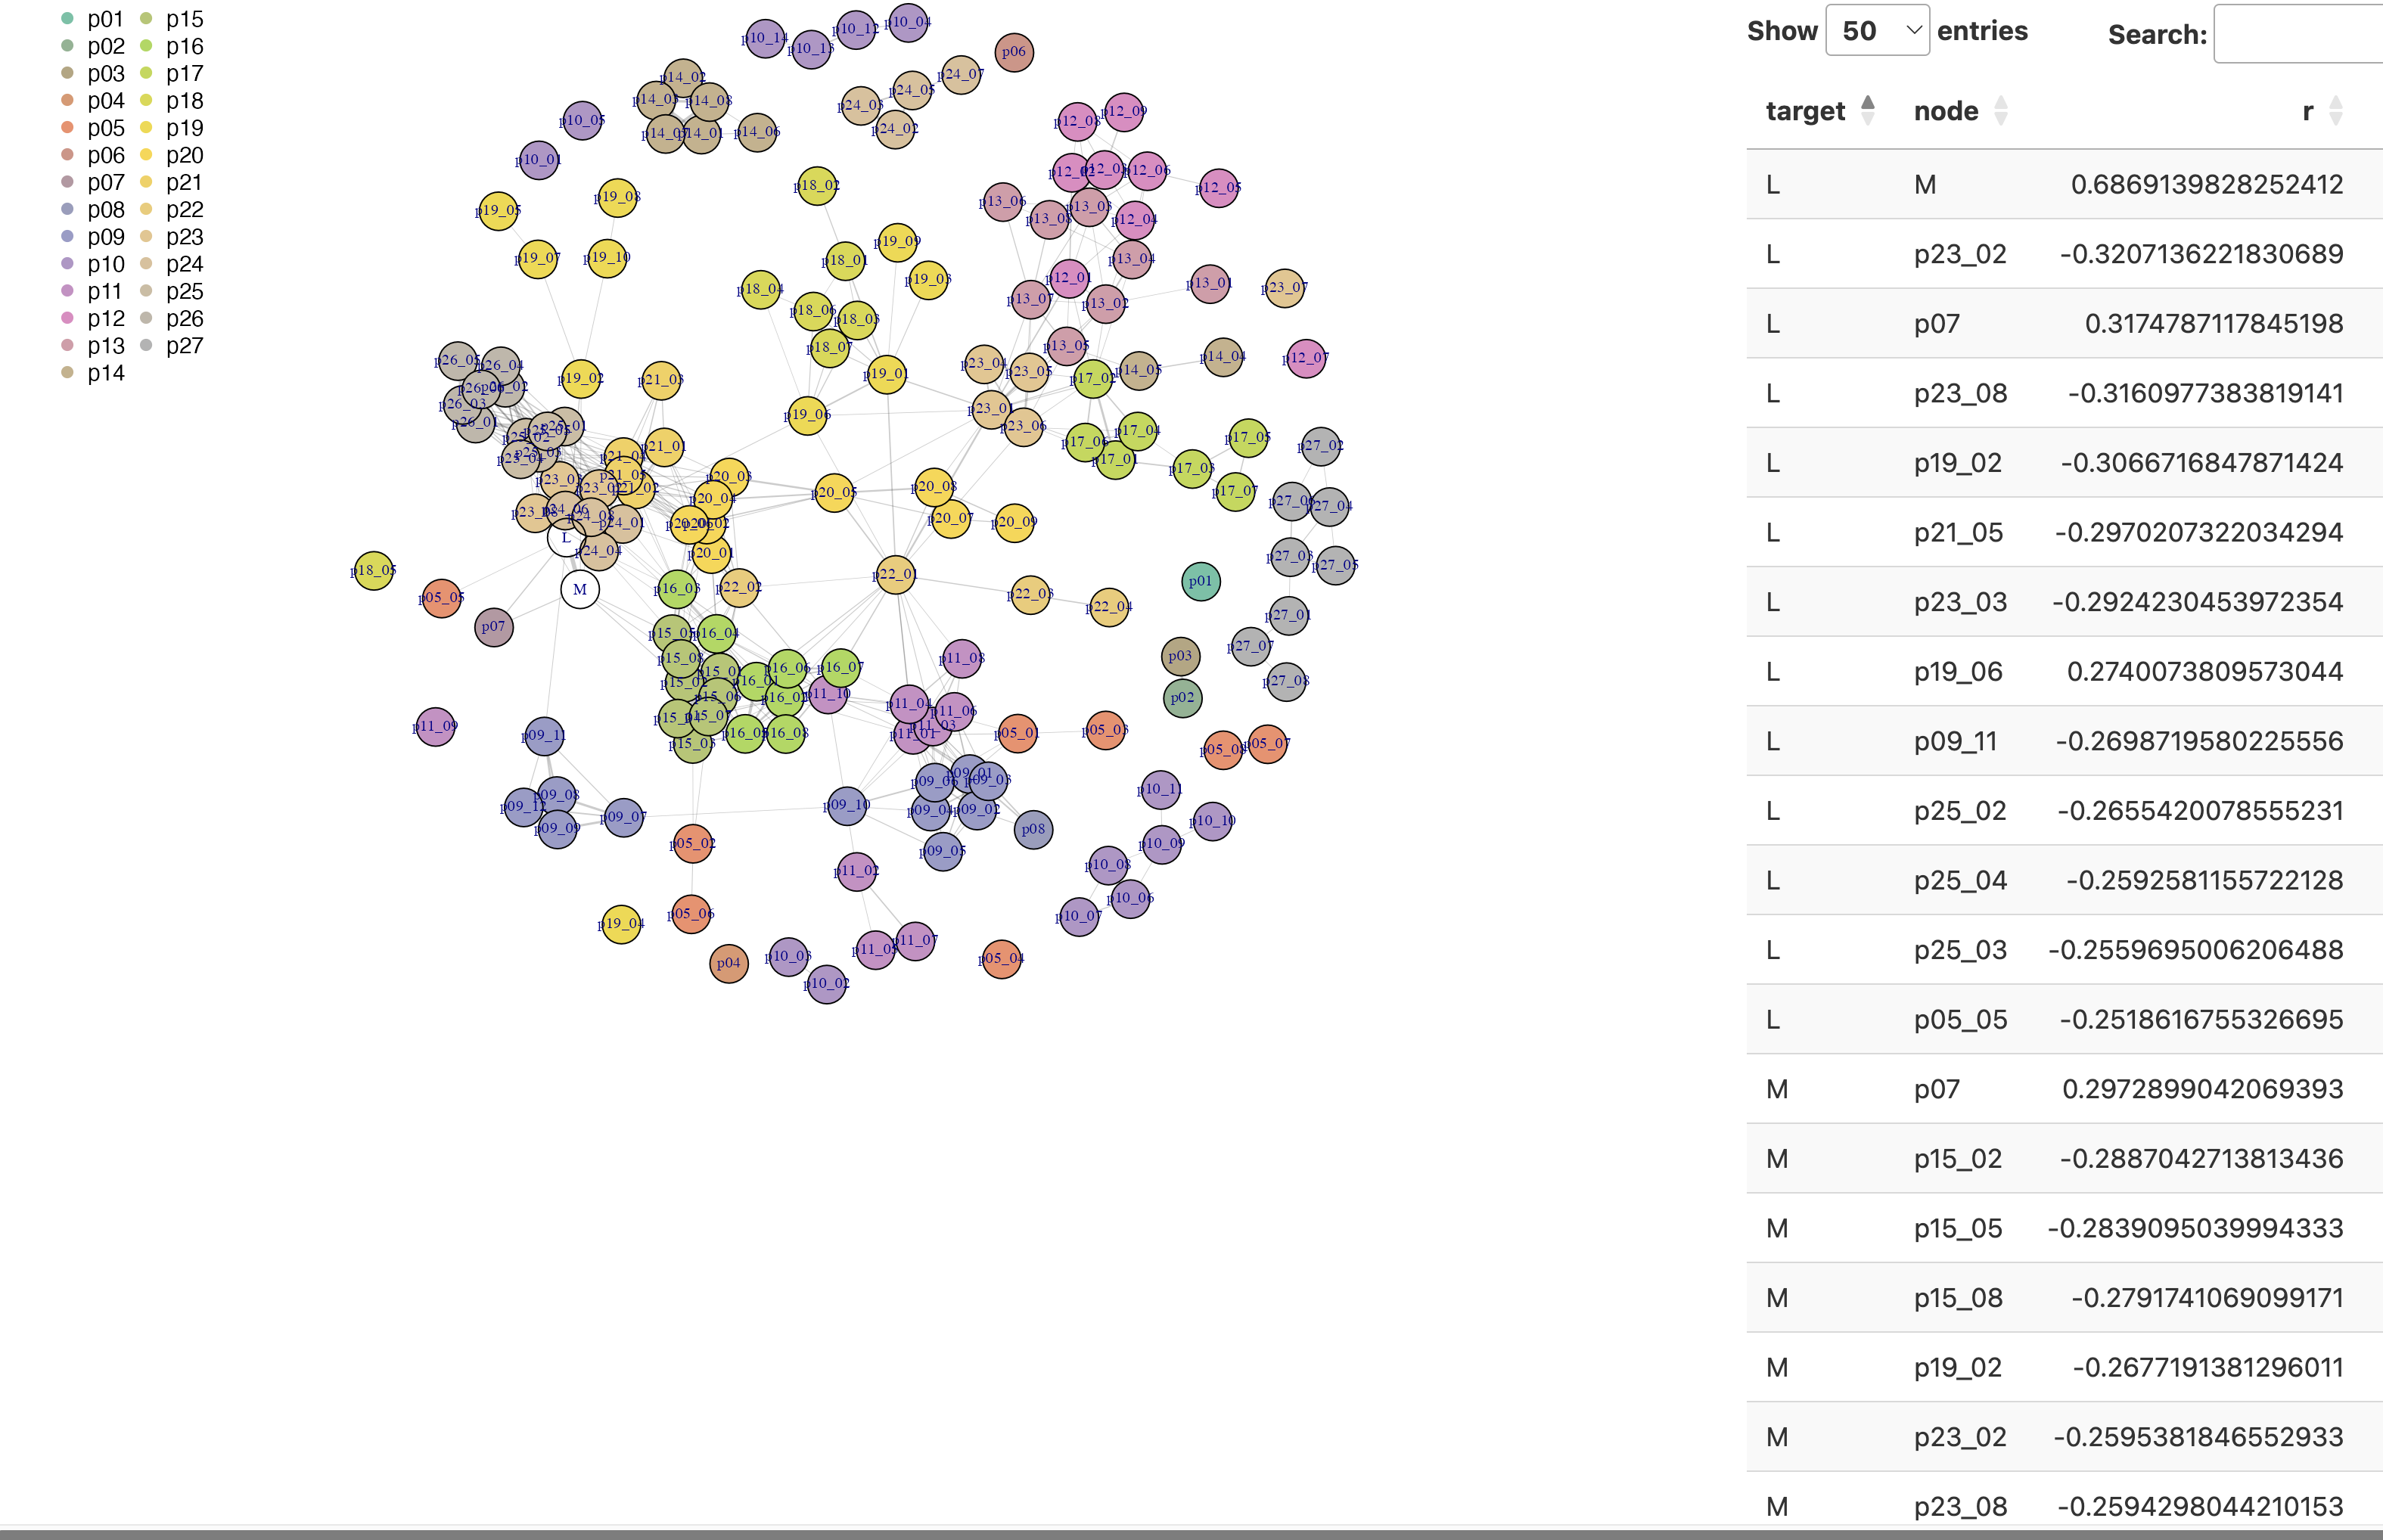
\includegraphics[width=0.9\textwidth]{figures/network_estudiante.png}}{\fbox{\begin{minipage}[c][0.3\textheight][c]{0.9\textwidth}\centering Placeholder: \texttt{figures/network\_estudiante.png} \end{minipage}}}
  \caption{Correlation network — Estudiante}
\end{figure}

\subsection{Familia}
\paragraph{Findings.}
At a glance, the Familia network highlights a tight coupling between Language (L) and Math (M). Predictors organize around two themes: (1) socio-educational capital and family involvement (e.g., support and learning routines at home, communication with the school), which relate positively to L/M; and (2) time-use and household stressors (e.g., excessive screen time, constraints at home), which relate negatively. This pattern is consistent with the idea that richer learning environments and higher expectations enable better outcomes.

In addition, the most salient family items point to parental education and expectations:
\begin{itemize}
  \item \textbf{Mother’s education:} ``¿Cuál es el nivel de estudios más alto que tiene la MADRE o APODERADA del estudiante?'' ("What is the highest level of education attained by the student's mother or female guardian?") Higher maternal education often proxies for socio-educational capital (literacy practices at home, academic expectations, ability to support homework), which is typically positively associated with both L and M.
  \item \textbf{Father’s education:} ``¿Cuál es el nivel de estudios más alto que tiene el PADRE o APODERADO del estudiante?'' ("What is the highest level of education attained by the student's father or male guardian?") Analogously, higher paternal education contributes resources, role modeling, and expectations that support academic performance.
  \item \textbf{Expected highest level for the student:} ``¿Cuál cree usted que será el nivel educativo más alto que alcanzará el estudiante?'' ("What do you believe will be the highest educational level the student will achieve?") Family expectations are a well-known driver of student aspirations, time devoted to study, and perseverance; in association networks, this tends to align positively with L/M.
\end{itemize}
Together, these indicators suggest that family socio-educational capital and expectations form a pathway linked to better outcomes, consistent with the observed positive links for p16/p02/p03 and the strong L–M correlation.

\subsubsection*{Causal Edges into Target}
% TODO
\begin{figure}[h]
  \centering
  \IfFileExists{figures/network_familia.png}{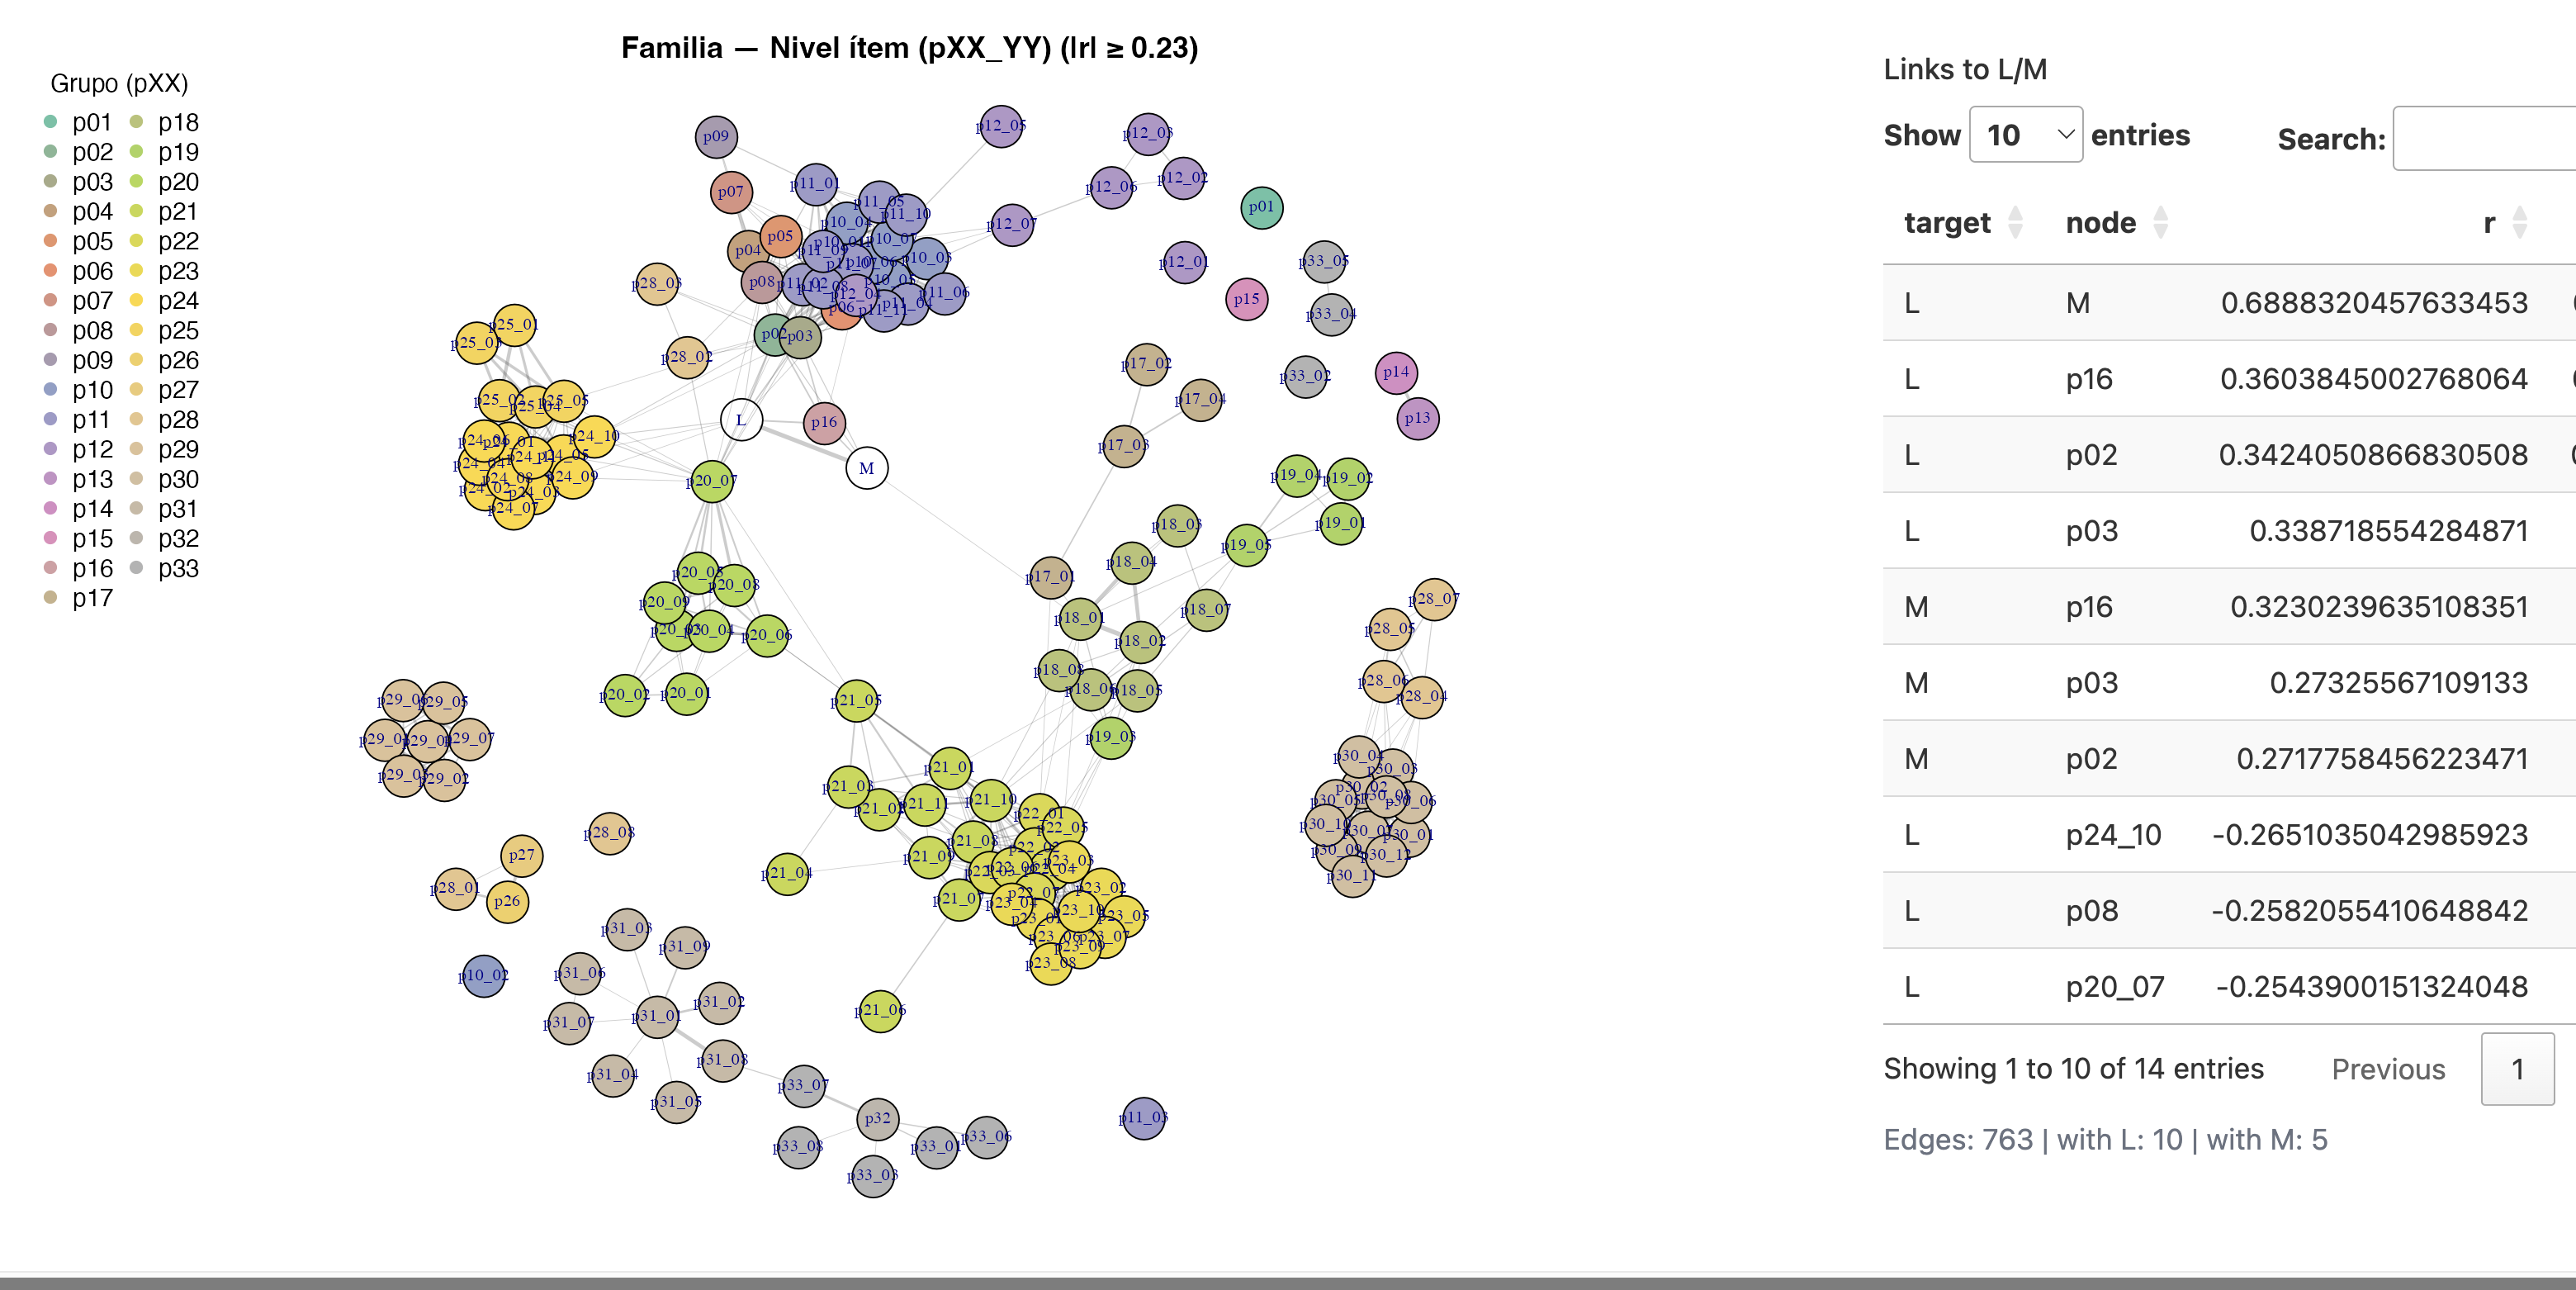
\includegraphics[width=0.9\textwidth]{figures/network_familia.png}}{\fbox{\begin{minipage}[c][0.3\textheight][c]{0.9\textwidth}\centering Placeholder: \texttt{figures/network\_familia.png} \end{minipage}}}
  \caption{Correlation network — Familia}
\end{figure}

\subsection{Docente Tutor}
\paragraph{Findings.}
L and M exhibit a strong positive correlation (r = 0.8608). Additional links into L include p14\_01 (0.2417) and a negative correlation for p01 (-0.2267). Two salient items in this source are:
\begin{itemize}
  \item \textbf{Student screen time (games):} ``En este último año, ¿cuántos estudiantes de su aula de 6.° grado de primaria han realizado alguna de estas acciones? Pasan 3 o más horas al día jugando videojuegos en el teléfono o la computadora.'' ("In the last year, how many students in your 6th-grade class have done the following? They spend 3 or more hours per day playing video games on a phone or computer.") Sustained daily gaming of 3+ hours typically displaces study time and sleep, and is often associated with reduced attention and homework completion. We therefore expect a \emph{negative association} with L/M at the aggregate class level.
  \item \textbf{Teacher years of experience:} ``¿Cuántos años de experiencia tiene usted como docente?" ("How many years of experience do you have as a teacher?") Greater experience can translate into more effective classroom management, feedback routines, and instructional repertoire, which should relate \emph{positively} to class performance. Effects may be nonlinear (e.g., diminishing returns), but the association in correlation networks is expected to be positive on average.
\end{itemize}

\subsubsection*{Causal Edges into Target}
% TODO
\begin{figure}[h]
  \centering
  \IfFileExists{figures/network_docente_tutor.png}{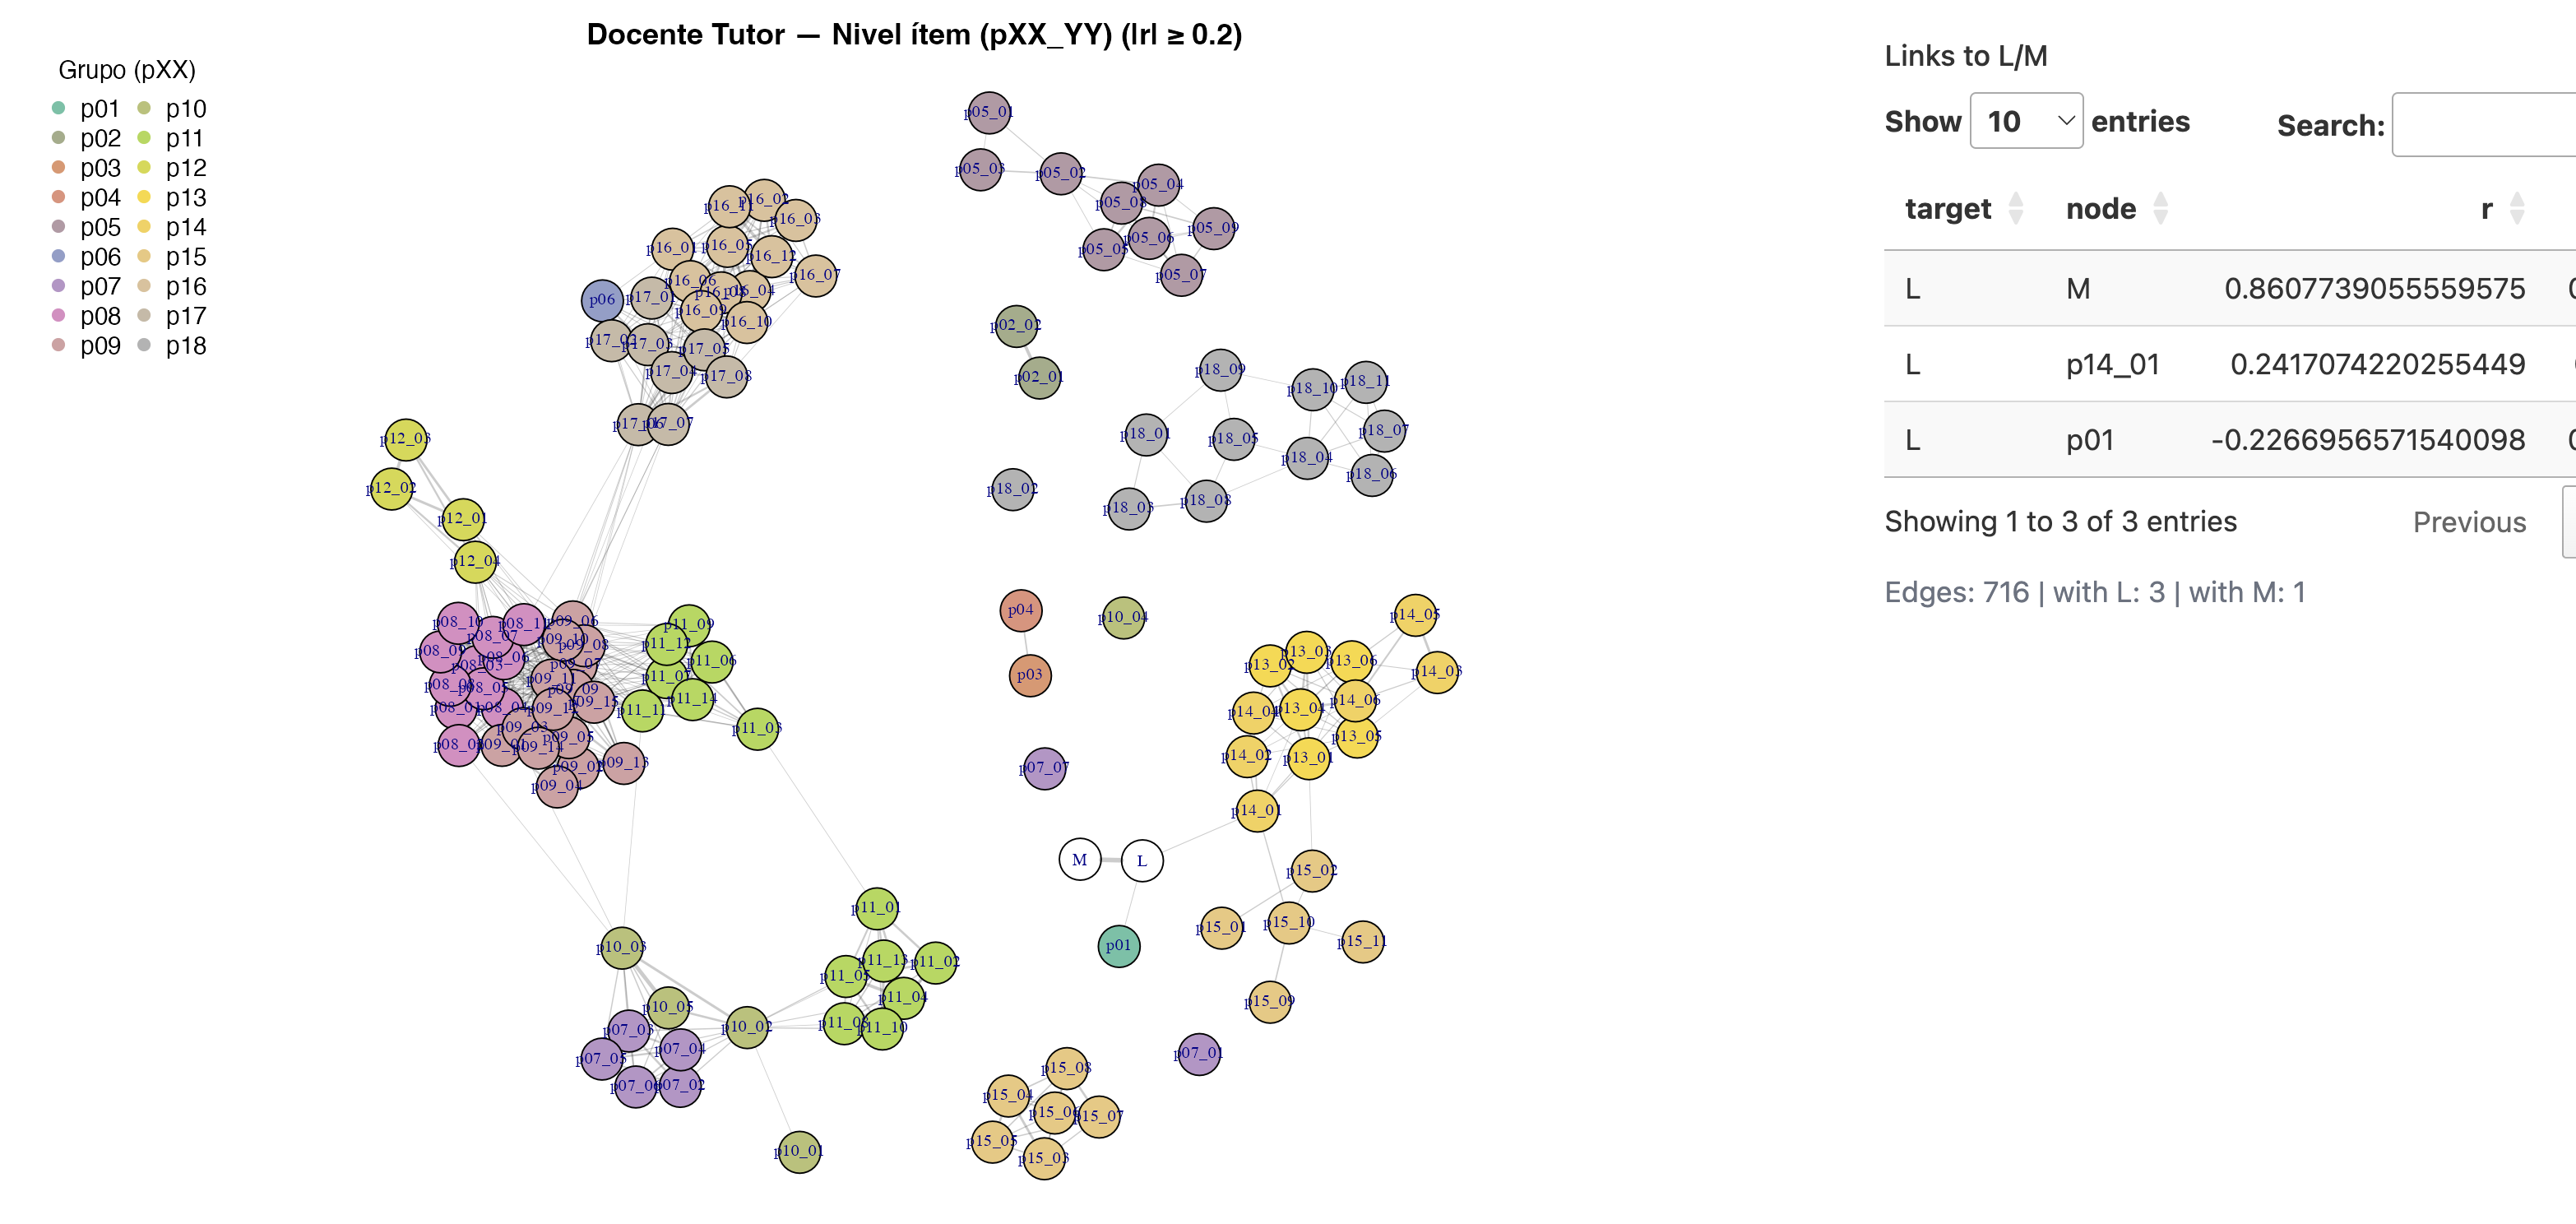
\includegraphics[width=0.9\textwidth]{figures/network_docente_tutor.png}}{\fbox{\begin{minipage}[c][0.3\textheight][c]{0.9\textwidth}\centering Placeholder: \texttt{figures/network\_docente\_tutor.png} \end{minipage}}}
  \caption{Correlation network — Docente Tutor}
\end{figure}

\subsection{Director F2}
\paragraph{Findings.}
Both outcomes show notable associations. Two school-level indicators stand out:
\begin{itemize}
  \item \textbf{Regular attendance (share of enrolled students attending regularly).} ``Aproximadamente, ¿qué porcentaje del total de estudiantes matriculados de primaria está asistiendo a clases de manera regular en el presente año?" ("Approximately, what percentage of total enrolled primary students are regularly attending classes this year?") Higher regular attendance expands instructional time and continuity, which should \emph{positively} relate to performance in both L and M.
  \item \textbf{Regional external evaluations in 4th grade.} ``Durante el presente año escolar, ¿cuántas veces su escuela ha tenido las siguientes actividades en 4.° grado de primaria? Evaluación de estudiantes organizada por la DRE o Gobierno regional." ("This school year, how many times has your school had the following activities in 4th grade? Student evaluations organized by the Regional Education Directorate or Regional Government.") Greater exposure can reflect an assessment culture and data use for improvement, potentially \emph{positive} if feedback is used formatively. However, effects can be context-dependent (e.g., test-prep without instructional support).
\end{itemize}

\subsubsection*{Causal Edges into Target}
% TODO
\begin{figure}[h]
  \centering
  \IfFileExists{figures/network_director_f2.png}{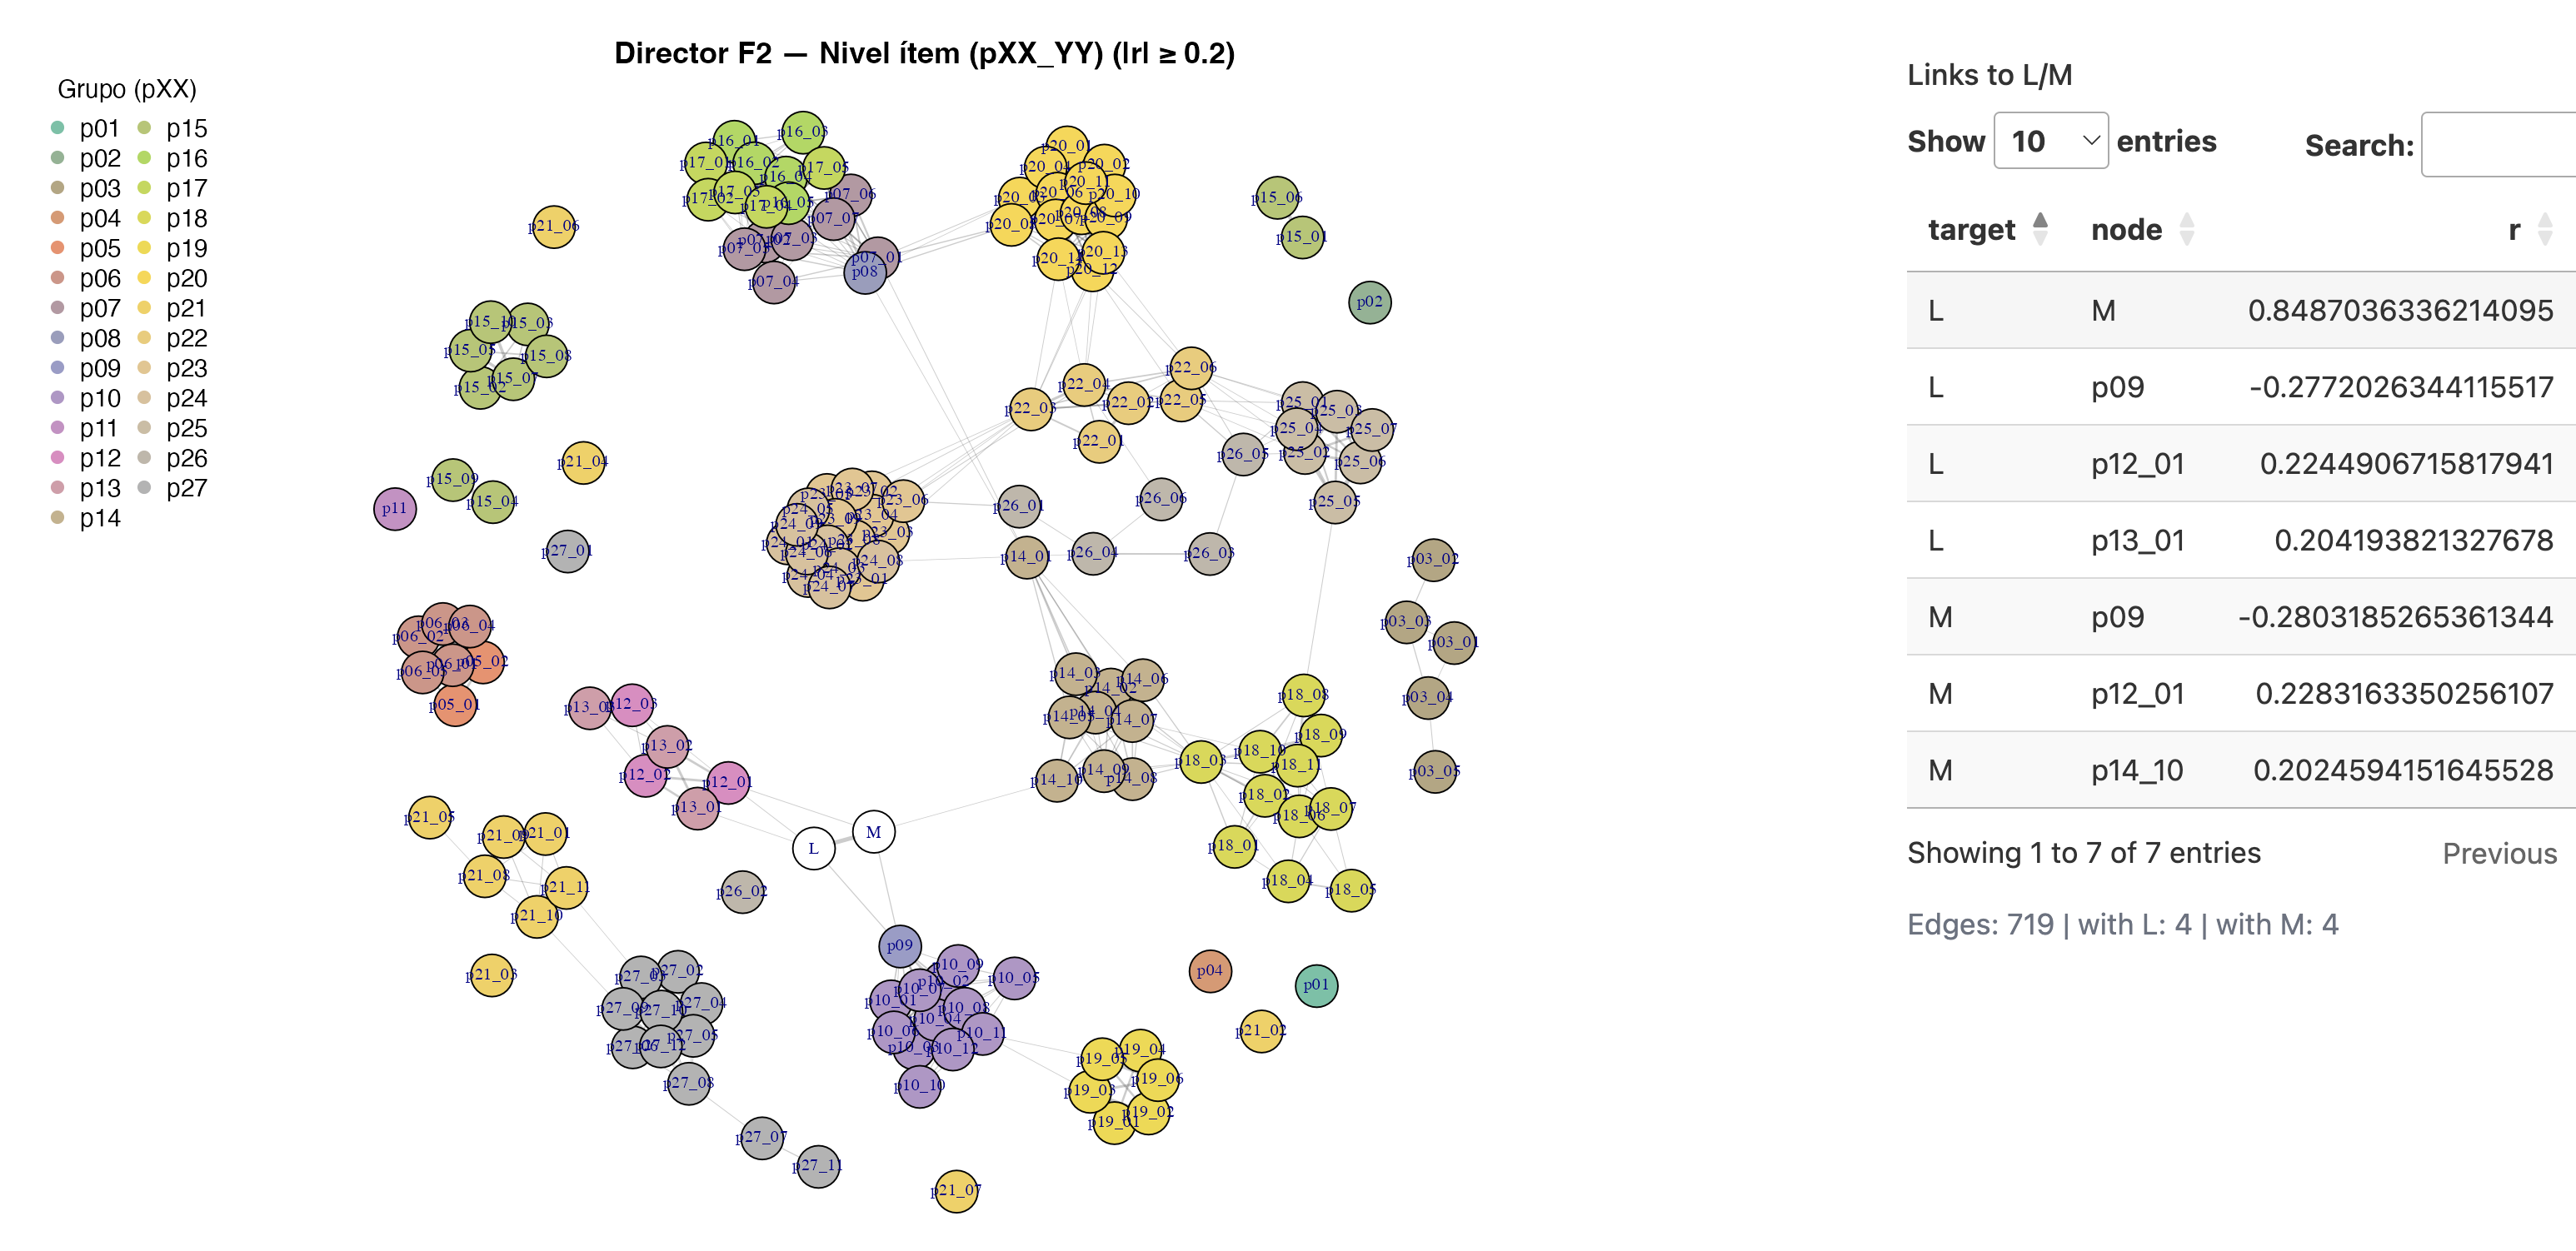
\includegraphics[width=0.9\textwidth]{figures/network_director_f2.png}}{\fbox{\begin{minipage}[c][0.3\textheight][c]{0.9\textwidth}\centering Placeholder: \texttt{figures/network\_director\_f2.png} \end{minipage}}}
  \caption{Correlation network — Director F2}
\end{figure}

\subsection{Docente Matemática}
\paragraph{Findings.}
Very strong L–M correlation (r = 0.8611). Two content/practice indicators appear particularly relevant for Math performance:
\begin{itemize}
  \item \textbf{Coverage of geometry topics (Angles in the plane; Elements and properties of quadrilaterals and triangles).} Given limited class time, reporting that these topics were covered with 6th graders likely reflects stronger pacing and curriculum coverage. Geometry strengthens spatial reasoning and deductive thinking; its systematic coverage should \emph{positively} relate to Math performance and can also support reading of mathematical text (diagrams, problem statements).
  \item \textbf{Teaching multiple subjects in addition to Math.} Besides Mathematics, do you also teach another area? Multi-subject teaching can have mixed implications: it may dilute time and specialization (potentially \emph{negative} for Math), but integrated pedagogy can also help transfer skills across domains. In association terms we often observe a small negative relationship with Math when teacher load is spread across several areas, contingent on school context.
\end{itemize}

\subsubsection*{Causal Edges into Target}
% TODO
\begin{figure}[h]
  \centering
  \IfFileExists{figures/network_docente_matematica.png}{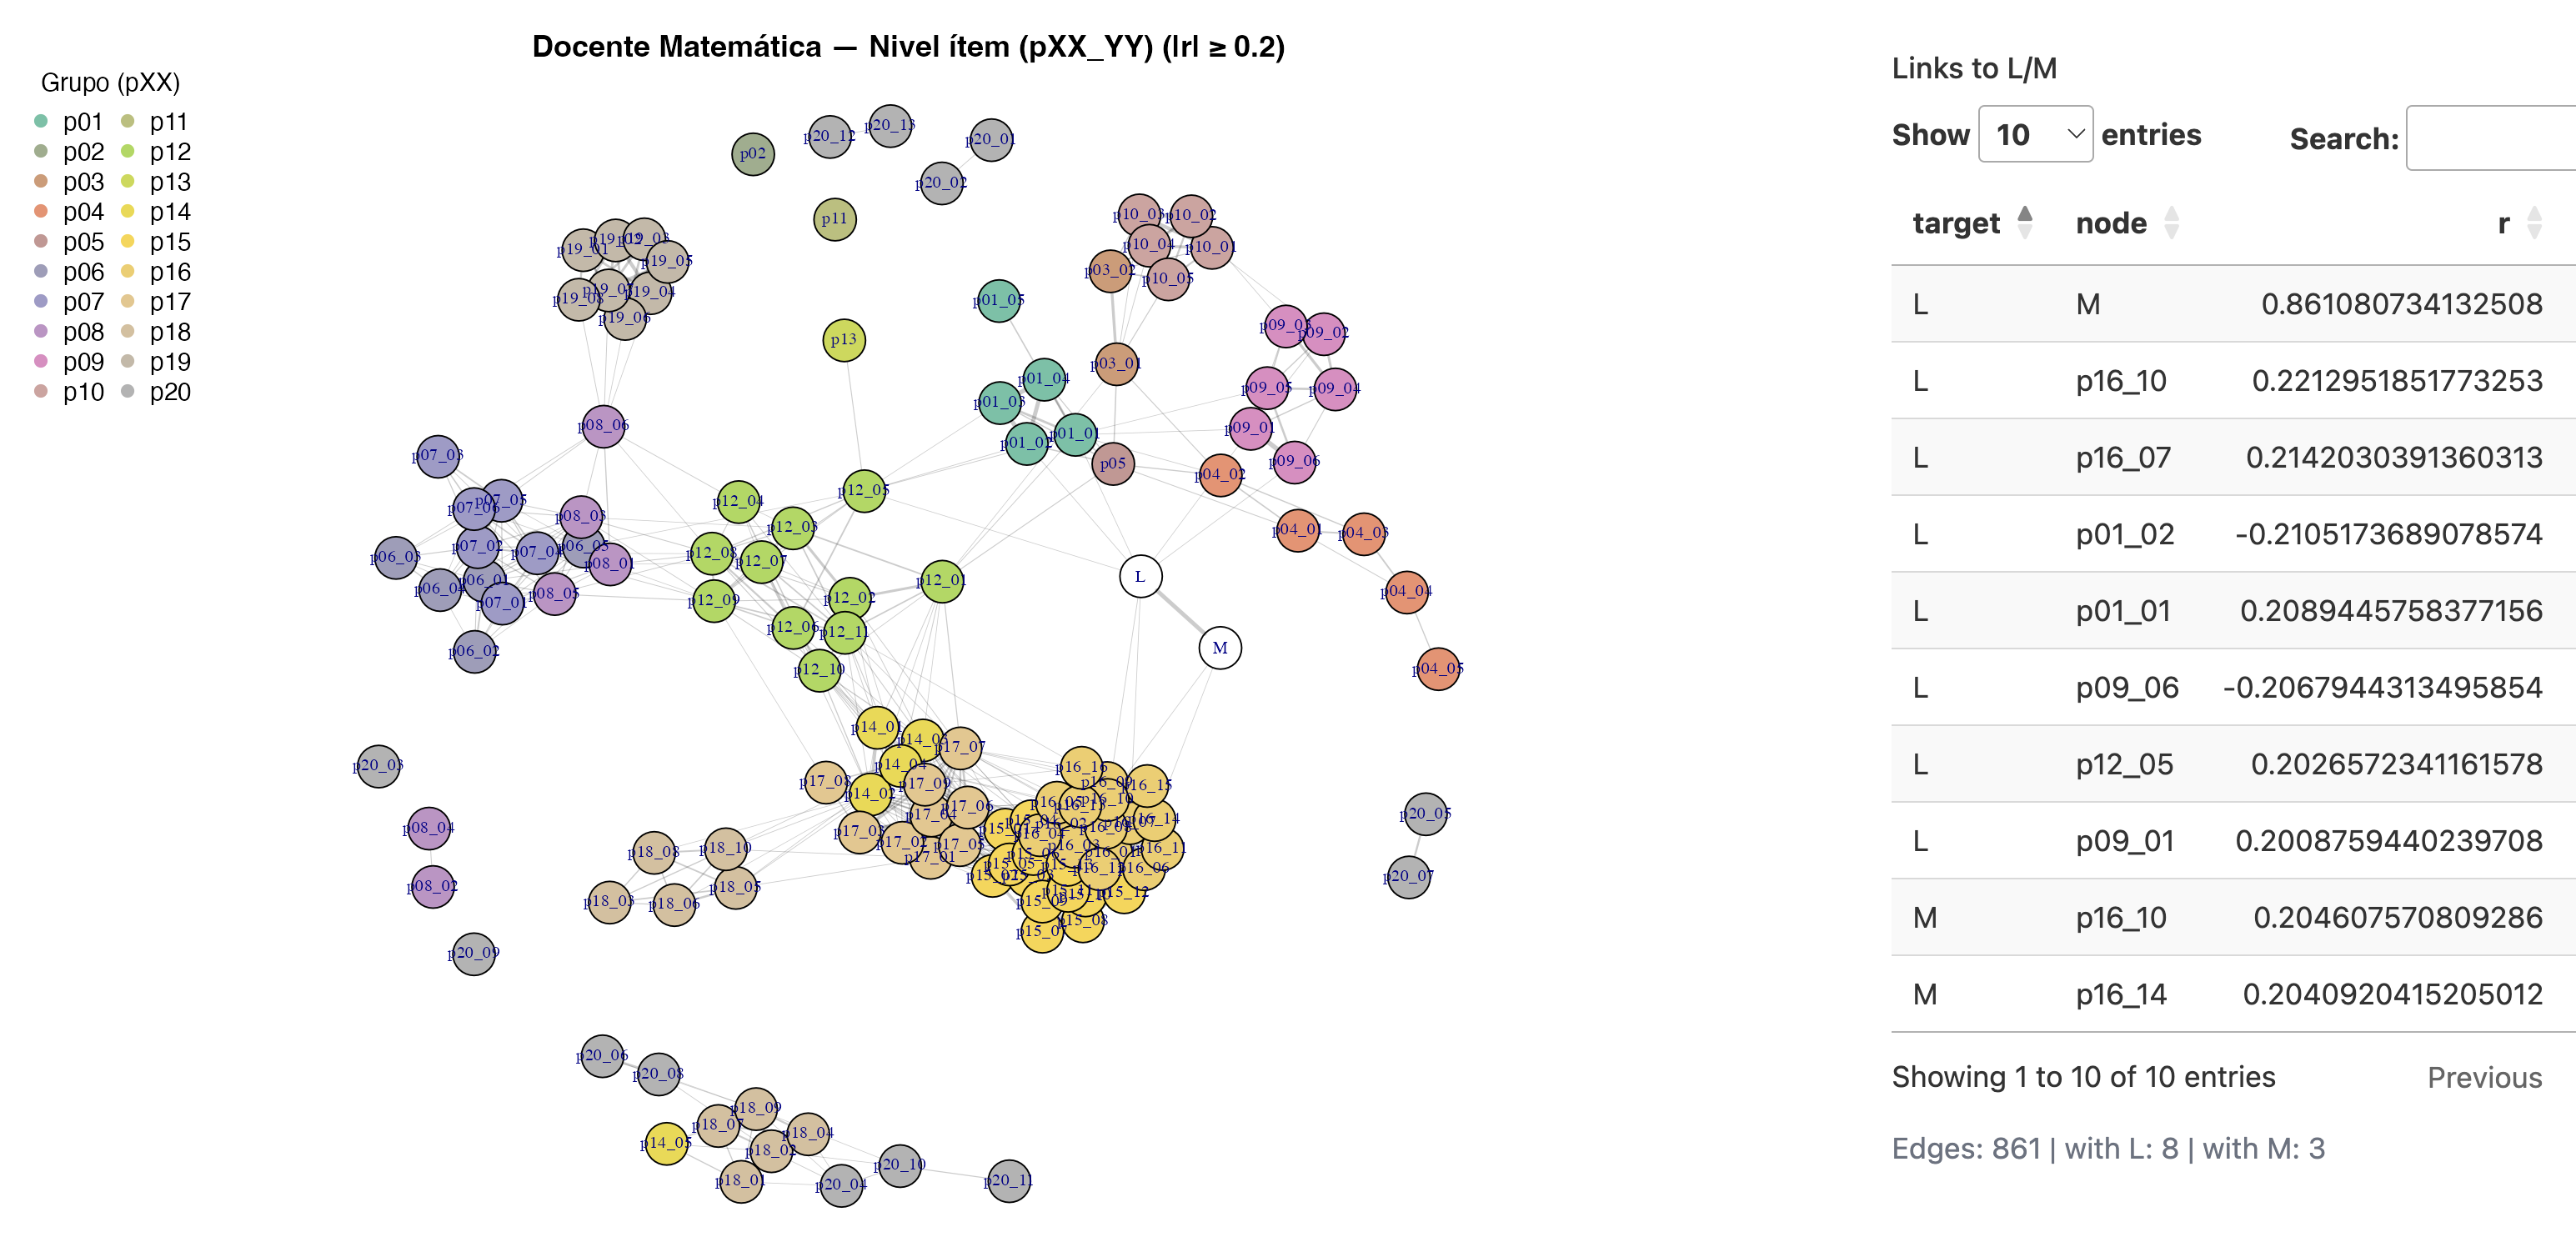
\includegraphics[width=0.9\textwidth]{figures/network_docente_matematica.png}}{\fbox{\begin{minipage}[c][0.3\textheight][c]{0.9\textwidth}\centering Placeholder: \texttt{figures/network\_docente\_matematica.png} \end{minipage}}}
  \caption{Correlation network — Docente Matemática}
\end{figure}

\subsection{Docente Comunicación}
\paragraph{Findings.}
Strong L–M correlation (r = 0.8611). Three items stand out in relation to performance:
\begin{itemize}
  \item \textbf{Sex:} We observe associations between sex and performance; this aligns with the EDA patterns where some subgroups differ in the upper tail of performance. Interpretation should be cautious and contextualized with opportunity-to-learn and classroom practices.
  \item \textbf{Use of books to select/prepare texts (for L):} This school year, how often have you used books to select or prepare texts for Communication class? More frequent use of book sources is plausibly linked to richer text selection and structured reading instruction, which should \emph{positively} correlate with Language performance.
  \item \textbf{If a student does not understand a text (for M):} If a student does not understand what a text is about, asking them to write on the board an explanation you dictate emphasizes transcription over comprehension monitoring or scaffolding strategies (e.g., re-reading, questioning, modeling inference). This may be \emph{negatively} associated with broader academic performance, including Math, as it reflects limited emphasis on meaning-making and problem-solving.
\end{itemize}

\subsubsection*{Causal Edges into Target}
% TODO
\begin{figure}[h]
  \centering
  \IfFileExists{figures/network_docente_comunicacion.png}{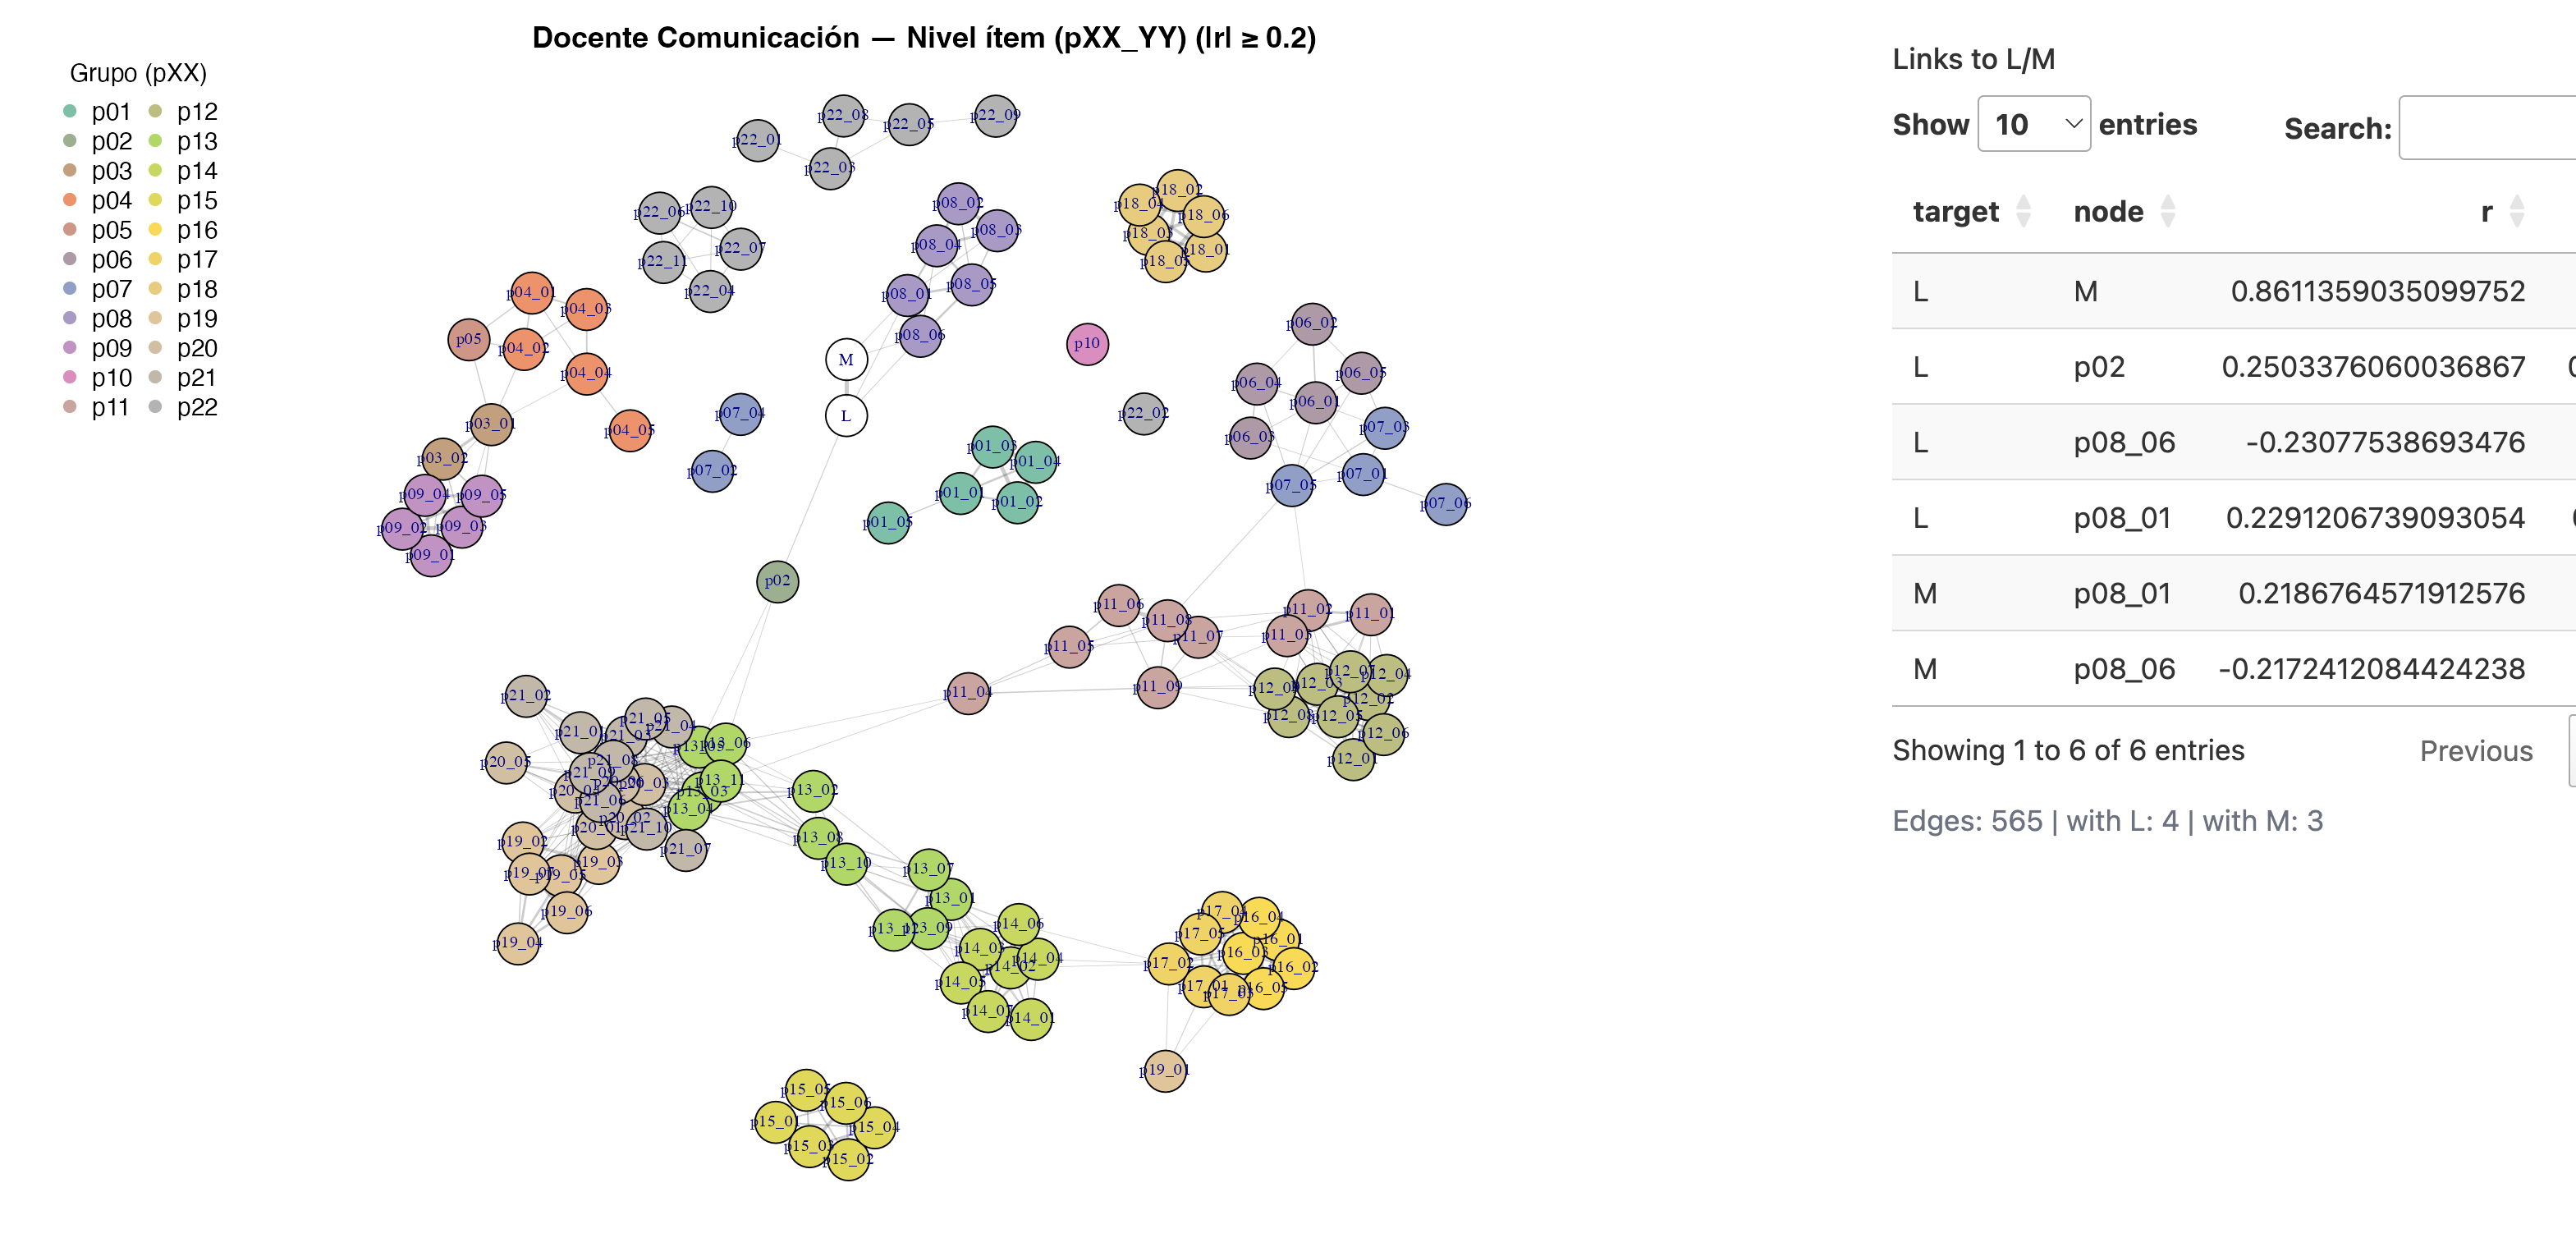
\includegraphics[width=0.9\textwidth]{figures/network_docente_comunicacion.png}}{\fbox{\begin{minipage}[c][0.3\textheight][c]{0.9\textwidth}\centering Placeholder: \texttt{figures/network\_docente\_comunicacion.png} \end{minipage}}}
  \caption{Correlation network — Docente Comunicación}
\end{figure}

% ===================== CAUSAL DISCOVERY =====================
\section{Causal Discovery}
We estimate directed acyclic graphs (DAGs) using the PC algorithm (constraint-based). PC proceeds in two stages: (i) it removes edges from an initially complete undirected graph by testing conditional independences, and (ii) it orients the remaining edges using v-structures and propagation rules (Meek rules).

\paragraph{Gaussian CI tests.}
Assuming joint normality, the conditional independence (CI) between two variables $X$ and $Y$ given a conditioning set $S$ is equivalent to a zero partial correlation $\rho_{XY\,\cdot S}=0$. Let $\Omega=\Sigma^{-1}$ be the precision matrix. For $S=\emptyset$, the partial correlation reduces to the correlation; for general $S$ one can compute $\rho_{XY\,\cdot S}$ via the precision of the submatrix:
\begin{equation}
  \rho_{XY\,\cdot S} 
  	= -\frac{\Omega_{XY}}{\sqrt{\Omega_{XX}\,\Omega_{YY}}}.
\end{equation}
In finite samples, significance is assessed with Fisher's $z$-transform
\begin{equation}
  Z\big(\rho_{XY\,\cdot S}\big)
  	= \frac{1}{2}\,\sqrt{n-|S|-3}\,\ln\!\left(\frac{1+\rho_{XY\,\cdot S}}{1-\rho_{XY\,\cdot S}}\right)
  \;\overset{H_0}{\sim}\; \mathcal{N}(0,1),
\end{equation}
and we declare CI if $|Z| < z_{1-\alpha/2}$.

\paragraph{Skeleton search.}
Starting from a complete undirected graph on variables $V$, PC removes edge $(X,Y)$ whenever it finds a set $S\subseteq N(X)\setminus\{Y\}$ (or symmetrically for $Y$) such that $X\perp\!\!\perp Y\mid S$ at level $\alpha$, beginning with $|S|=0$ and increasing $|S|$ until no more removals occur.

\paragraph{Orientation.}
For any unshielded triple $X\!\! -\! Z\! -\!\! Y$ with $X$ and $Y$ non-adjacent and $Z\notin S_{XY}$ (a separating set), orient a v-structure $X\to Z\leftarrow Y$. Then apply Meek rules to propagate orientations without creating cycles or new v-structures. The output is a CPDAG that represents the Markov equivalence class of DAGs consistent with the CI relations.

\paragraph{Implementation details.}
We use pairwise-complete covariances to build $\hat\Sigma$, mean-impute residual missingness, and select $\alpha$ based on stability. Targets (L/M) are highlighted when reporting incoming edges.

\subsection*{Student-level findings (incoming edges into L/M)}
At the student questionnaire level, PC identified the following variables as direct parents into the targets (L and/or M). Below we list the prompt and an interpretation of the expected relationship:
\begin{itemize}
  \item \textbf{First language learned:} ``¿Cuál fue la primera lengua que aprendiste a hablar?'' ("What was the first language you learned to speak?") Language background can influence early literacy exposure and access to instruction; associations often reflect advantages for Spanish as a first language in Spanish-medium schooling.
  \item \textbf{Recent absences:} ``Durante el último mes, ¿cuántos días has faltado a la escuela?" ("In the last month, how many days have you missed school?") More absences reduce instructional time and continuity, typically showing a \emph{negative} relation with L/M.
  \item \textbf{Reading time in free time:} ``En una semana habitual, ¿cuántas horas les dedicas a la lectura en tu TIEMPO LIBRE?" ("In a usual week, how many hours do you spend reading in your free time?") More voluntary reading is commonly \emph{positively} related to Language and, indirectly, to Math via problem comprehension.
  \item \textbf{Math anxiety (blank mind):} ``¿Qué tan de acuerdo estás con las siguientes afirmaciones? Cuando hago problemas de matemática se me pone la mente en blanco y no puedo pensar claramente." ("When I do math problems my mind goes blank and I cannot think clearly.") Higher agreement signals math anxiety/cognitive interference and is expected to be \emph{negatively} associated with M (and sometimes L through test anxiety).
  \item \textbf{Rote emphasis in Personal Social:} ``¿Qué tan seguido el profesor o profesora que enseña PERSONAL SOCIAL hace lo siguiente? Nos pide aprender de memoria los hechos tal como los explicó." ("How often does the Personal Social teacher ask students to memorize facts exactly as explained?") Stronger rote emphasis can crowd out comprehension/inference strategies; associations tend to be \emph{negative}, especially for transfer tasks.
  \item \textbf{School belonging (loneliness):} ``Acerca de tu escuela, ¿qué tan de acuerdo estás con las siguientes afirmaciones? Mi escuela es un lugar donde me siento solo." ("About your school, how much do you agree: My school is a place where I feel lonely.") Higher loneliness indicates lower belonging/support and is typically \emph{negatively} related to performance.
  \item \textbf{Classroom discipline climate (disrespect toward teachers):} ``¿Qué tan de acuerdo estás con las siguientes afirmaciones acerca de tus profesores? Los profesores dejan que los estudiantes les respondan de forma inadecuada o insulten." ("Teachers allow students to answer them inappropriately or insult them.") Weak disciplinary climate undermines instructional time and expectations; a \emph{negative} relation with L/M is expected.
  \item \textbf{Teacher listening with interest:} ``Durante las clases, ¿qué tan seguido tus profesores hacen lo siguiente? Nos escuchan con interés cuando opinamos en clase." ("During class, how often do your teachers listen with interest when we share our opinions?") Supportive engagement is associated with participation and feedback; a \emph{positive} relation with L/M is expected.
\end{itemize}

% Place causal discovery example after the questionnaire section
\begin{figure}[h]
  \centering
  \IfFileExists{figures/causal_discovery_example.png}{%
    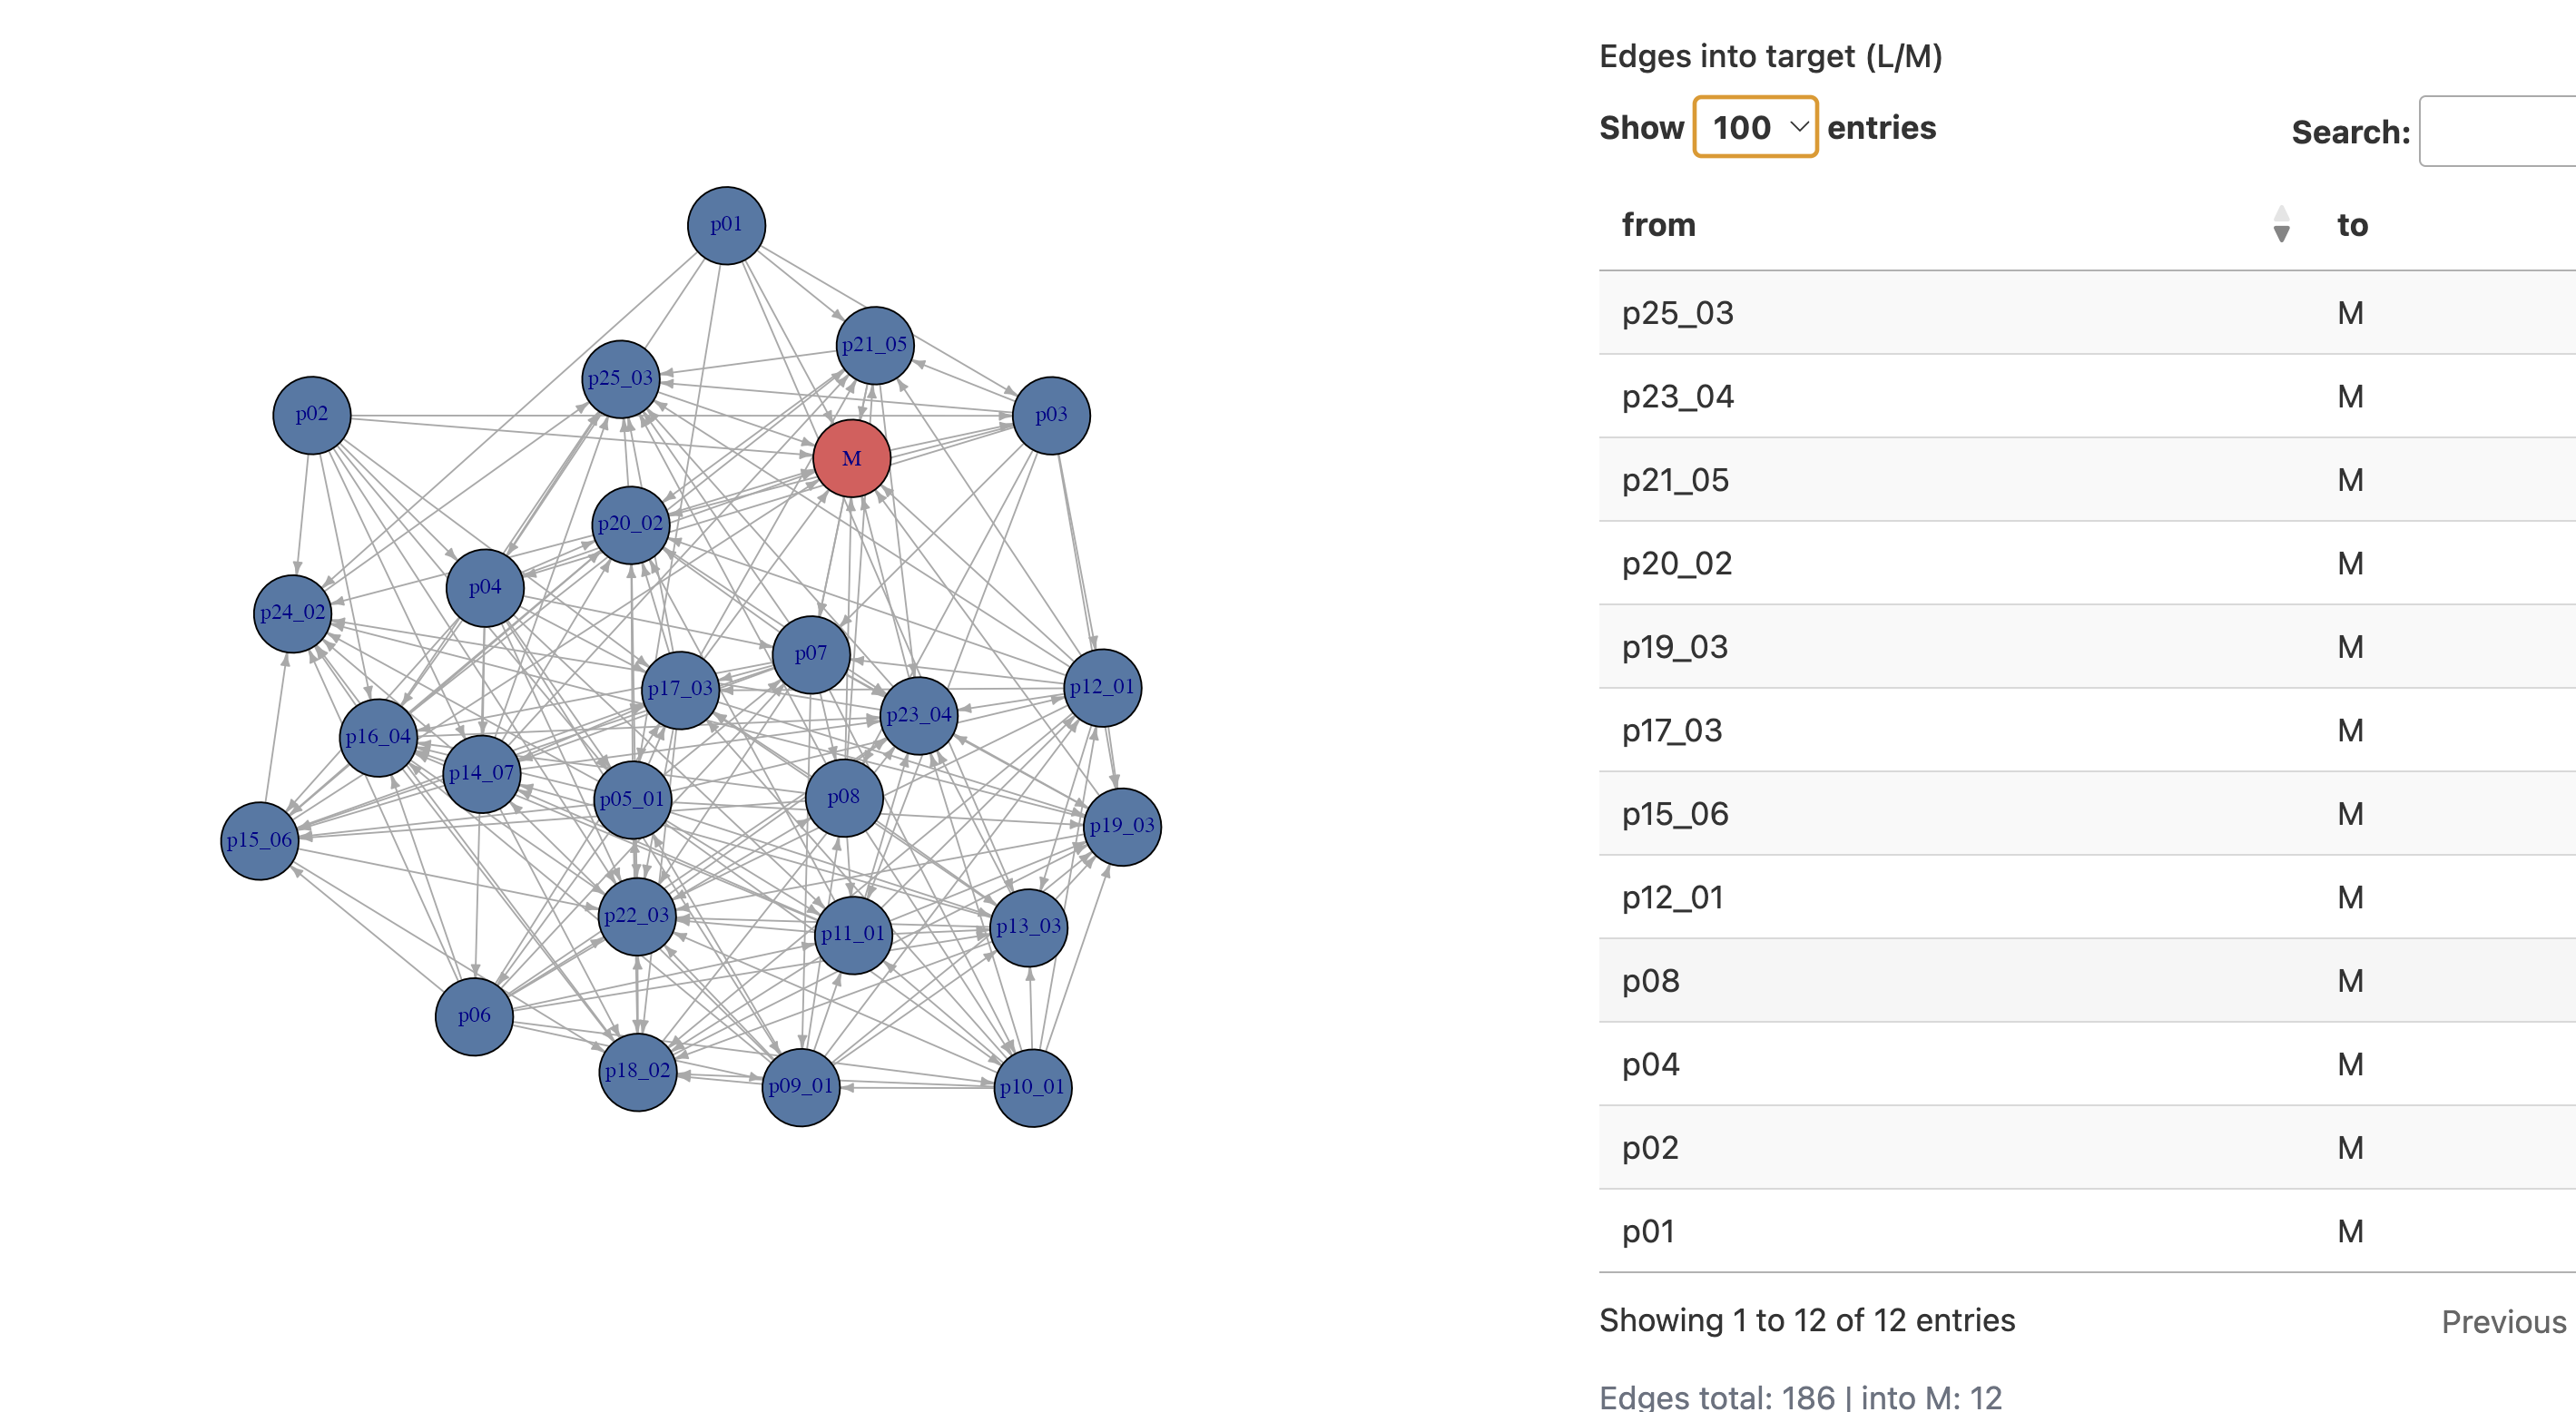
\includegraphics[width=0.9\textwidth]{figures/causal_discovery_example.png}%
  }{%
    \fbox{\begin{minipage}[c][0.3\textheight][c]{0.9\textwidth}\centering
    Placeholder: \texttt{figures/causal\_discovery\_example.png}
    \end{minipage}}%
  }
  \caption{Example causal discovery result (PC algorithm) with target highlighted.}
\end{figure}


\end{document}
